\documentclass[12pt]{article}

\usepackage{graphicx,amsmath}
\usepackage[margin=1in]{geometry}
\usepackage{float}

\title{CMDA 3634 PSA03 : MPI $k$-center}
\author{Jason Bruno Terceros}
\date{\today}

\begin{document}

\maketitle

In this write-up we consider running our OpenMP $k$-means on ARC. We will also be implementing our code by making it parallel and using static scheduling. This will be done by adjusting two functions in code that is provided to us. Finally, we will run our code and produce images out to visually see how our code produced these images on ARC.


\section{The $k$-Center Problem}

Given n points \textbf{$p_1, p_2, . . . , p_n$} in $d$-dimensional space, the objective of the $k$-center problem is to choose $k$ center points \textbf{$c_1, c_2, . . . c_k$} from the list of $n$ given points so that the \textbf{maximum distance} between any point and its \textbf{closest} center is \textbf{minimized}. Mathematically speaking, we wish to choose $k$ center points \textbf{$c_1, c_2, . . . c_k$} to minimize the following \textbf{cost} function.

\begin{equation}
\text{cost($c_1, c_2, ... , c_k$)} = 
\displaystyle \max _{1\leq i \leq n }\min ( \left\|\mathbf {p}_{i} -{\mathbf{c}}_{1}\right\|^2 , \left\|\mathbf {p}_{i} -{\mathbf{c}}_{2}\right\|^2, ..., \left\|\mathbf {p}_{i} -{\mathbf{c}}_{k}\right\|^2 )
\end{equation}

Suppose we want to solve the 8-center problem on a dataset with $n$ = 120 cities. Since $\tbinom {120}{8}$ = 840261910995, a brute force algorithm for solving the 8-center problem exactly would require a lot of computation time. In this assignment you are given the source code for a complete sequential C program that implements an approximation algorithm (with the distance lookup table and early abort optimizations) for solving the $k$-center problem by randomly selecting and checking $m$ different sets of $k$ center locations. The dataset filename, values of $k$, $m$ as well as the random seed $s$ are read in as command line arguments. You will write a \textbf{parallel version} of the given $k$-center program \textbf{using MPI}. For this assignment we will use parallel computing to enlarge the number of sets of random center locations checked rather than reduce the overall runtime. In particular, \textbf{each rank will check $m$ different sets of $k$ center locations. For this assignment, you will develop and test your MPI code on ARC.}


% end of k-center probelm section

\section{Implementation Tasks}

For our implementation, we will be modifying the provided mpi\_kcenter.c to implement the randomized $k$-center algorithm in parallel using MPI. 
We had to copy the files from \textasciitilde/cmda3634\_materials/PSA03 to my private directory on ARC.  

\begin{enumerate}
\item Coding Tasks
In the dataset, values $k$, $m$ as well as the random seed $s$ are read in as command line arguments. \textbf{Each rank will check $m$ different sets of $k$ center locations.}
To prevent each rank from testing the same m sets of k centers, \textbf{add $rank$ to the random seed $s$.}

As such, my implementation outputs the following requirements:
    \begin{enumerate}
    \item Wall time used
    \item Total number of tuples checked (\textbf{in the MPI version, each rank checks m random tuples}).
    \item Overall approximate minimal cost
    \item Overall approximate optimal centers
    \end{enumerate}
We were also informed that we must use MPI point-to-point communication 
\textbf{($i.e.$ MPI\_Send and MPI\_Recv) in order to find the overall approximate optimal cost and center indices.}

Attached here is my implemented code:

\begin{verbatim}
srandom(atoi(argv[4]) + rank);
if (rank == 0)
{

    for (int src = 1; src<size; src++)
    {
        double rmcs = DBL_MAX;
        MPI_Status status;
        MPI_Recv(&rmcs, 1, MPI_DOUBLE, src, 0, MPI_COMM_WORLD, &status);
        MPI_Recv(centers, k, MPI_INT, src, 0, MPI_COMM_WORLD, &status);

        if (rmcs < min_cost_sq)
        {
            min_cost_sq = rmcs;
            for (int i = 0; i<k; i++)
            {
                optimal_centers[i] = centers[i];
            }
        }
    }
}
else
{
    int dest = 0;
    MPI_Send(&min_cost_sq, 1, MPI_DOUBLE, dest, 0, MPI_COMM_WORLD);
    MPI_Send(optimal_centers, k, MPI_INT, dest, 0, MPI_COMM_WORLD);
}
\end{verbatim}

\item Testing Tasks

Now we need to test and debug our script. So we need to call mpi\_kcenter\_debug.sh. This test is found in the materials repo that I will run using sbatch (provided to me) to test my code on a set of 120 cities.
My output:

Figure  
\ref{image1.fig} 
shows my command line run to have my output. Figure \ref{image1.fig} also show my output values. 
My command prompt outputs are:
\begin{verbatim}
[jasob19@tinkercliffs2 PSA03] 
" "           $ sbatch mpi_kcenter_debug.sh cities120.dat 8 20000000 20
Submitted batch job 2318094
[jasonb19@tinkercliffs2 PSA03]$ cat mpi_kcenter_debug.out
wall time used = 2.7582 sec
total number of 8-tuples checked = 160000000
approximate minimal cost = 1.9693
approximate optimal centers : 89 97 99 46 50 9 76 32
\end{verbatim}

\begin{figure}[H]
\begin{center}
    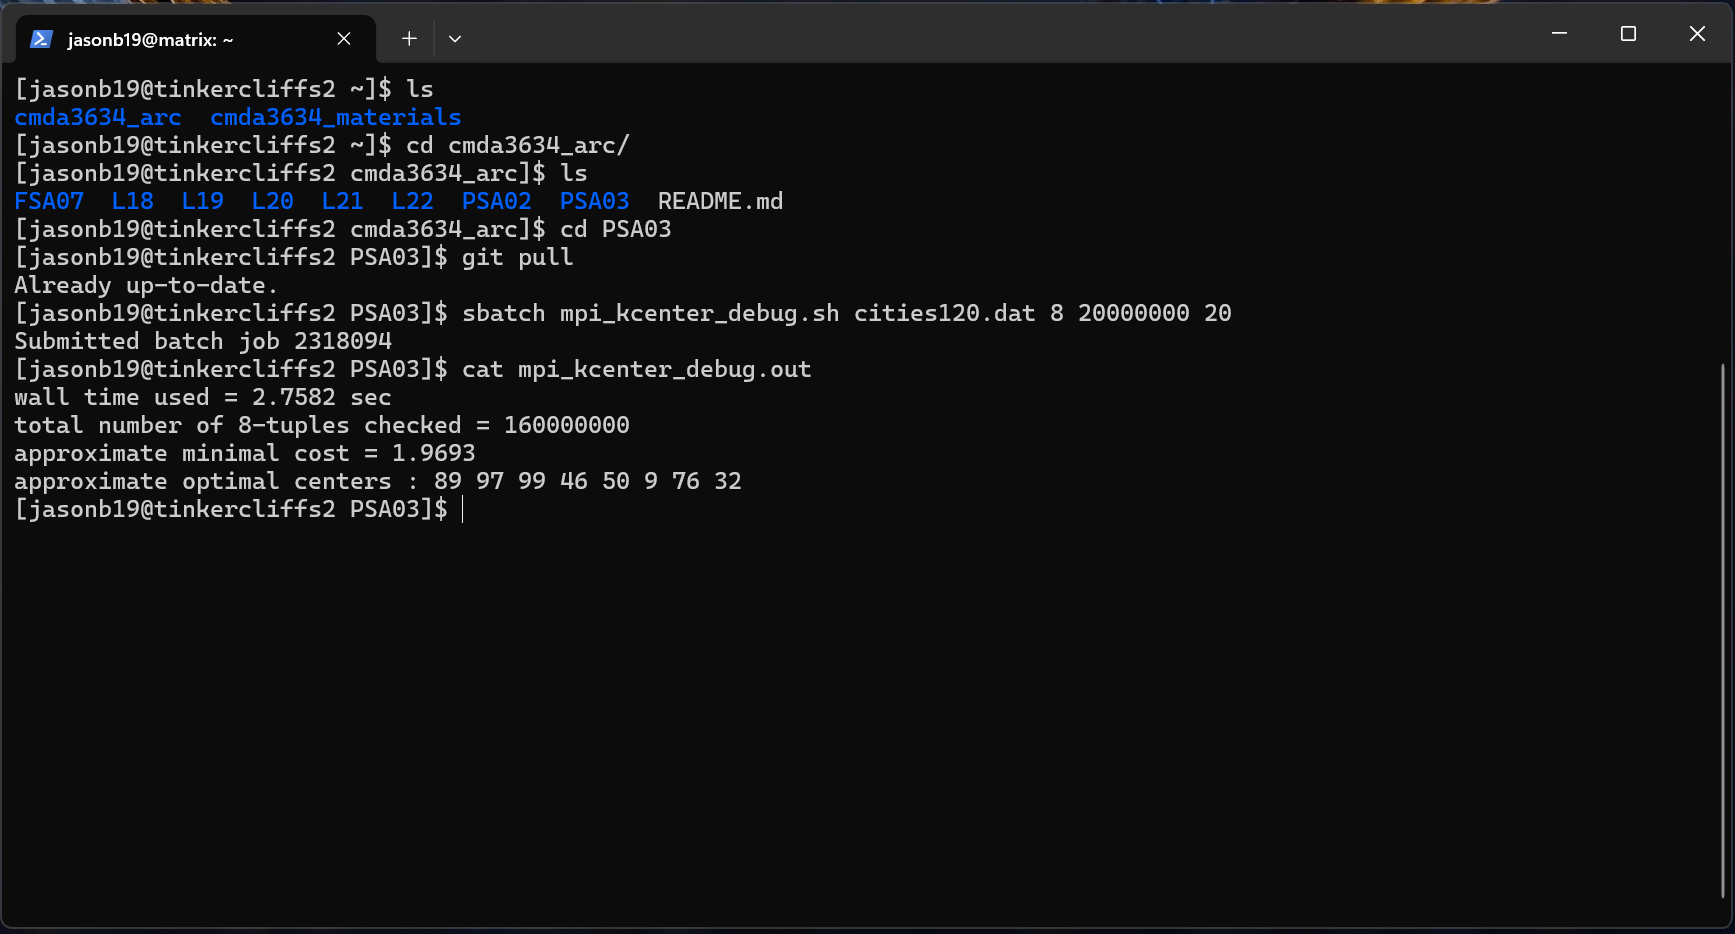
\includegraphics[width=0.95\textwidth]{images/image1.png}
\end{center}
\caption{ARC Command $k$=8, $m$=2M, and $s$=20}
\label{image1.fig}
\end{figure}


Figure \ref{cities120_8.fig} is my python image output. This image produces the optimal k-centers for each of the 120 data points.
 
\begin{figure}[H]
\begin{center}
    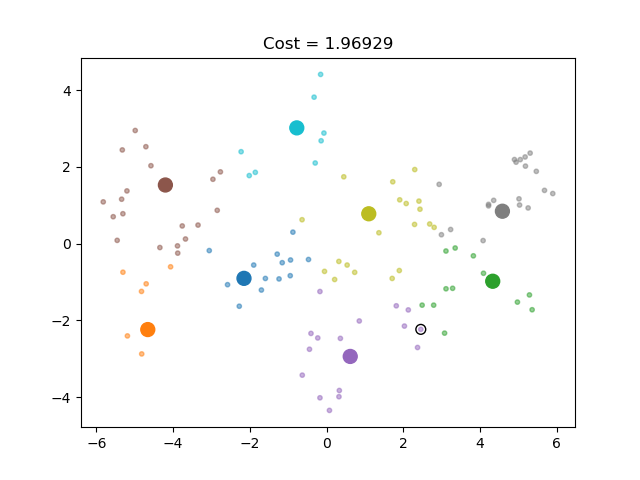
\includegraphics[width=0.95\textwidth]{images/cities120_8.png}
\end{center}
\caption{An Optimal Image for $k$=8, $m$=2M, and $s$=20}
\label{cities120_8.fig}
\end{figure}

\end{enumerate}

% end of Implementation tasks section

\section{Conceptual Write-Up Tasks}

Conceptual Write-Up Questions


\begin{enumerate}
\item How many different sets of 8 centers will have to be checked? Assuming that the program can check 10 million sets of 8 centers per second, how many hours will it take to check all possible sets of centers?

I am not sure If I understand this properly. But I will give it a go, so I am assuming this is would be 10 million per set. This would get me 80 millions to check. With 120 cities using $k$=8, $m$=20M, and seed is 20. Given this information, I assume It would be $k$=8, $m$=80M. Sop I will use this time constant to figure out how long it will run to get these results. The wall time for $k$=8, $m$=20M is 2.7582 seconds. 

\item What is the big advantage of using MPI over OpenMP?

MPI is more flexible and scalable than OpenMP, as you can run the program on any different number of processes that we wish to provide it. This includes, but is not limited to, memory sharing and process communication. For example, OpenMP, begins as sequential code and then runs in paralle and then back in sequential. This OpenMP is constantly sharing memory. However, in MPI processing, we get full parallel coding where we do not have to share or split any memory to run our program. Then, at the end we effectively communicate with our processors and share information rather than compiling the code all together.

\item Describe three major differences between MPI and OpenMP.

The main differences I believe exist from these two is programming, memory, and parallelism granularity. MPI follows the message passing programming model. This is where communication is achieved through message passiong operations. While OpenMP follows the shared-memory programming model, where multiple threads of execution share the same address space. MPI is suitable for distributed memory systems, where each process has its own memory space. While OpenMP is designed for shared-memory systems. This is where multiple threads have access to a common address space. Finally, MPI provides fine parallelize computations at the processor level. This is where developers have full control over the parallelism which can provide them with more efficient use of resources. While, OpenMP provides coarse parallelism which primarily focuses on usiung loops, regions, and tasks that can share-memory with the system.

\item What do these lines in mpi\_kcenter\_debug.sh script specify?

lines:
\begin{verbatim}
#SBATCH –nodes=2
#SBATCH –ntasks-per-node=4
\end{verbatim}

Since we are running in MPI, I believe we are telling it to use two processors. And for each processor we are running four simultaneous runs in each of these processors at the same time.

\item What does the command line argument to the mpicc compiler -O3 specify in the mpi\_kcenter\_debug.sh script? Why should we use this command line argument to help us search for the optimal k-center solution?

From what I understand -03 is a way for us, the user, to compile something to the highest level of optimization to our compiler. Overall, leveraging the -O3 optimization level with the mpicc compiler helps to enhance the efficiency and effectiveness of the k-center search algorithm, ultimately leading to faster convergence towards the optimal solution.

\item How many MPI ranks are used during execution of the mpi\_kcenter\_debug.sh test script?
\begin{verbatim}
#SBATCH --nodes=2
#SBATCH --ntasks-per-node=4
\end{verbatim}
So I believe as a tester, I believe we are running 4 ranks for this.

\item How many MPI ranks are used during execution of the mpi\_kcenter\_search.sh test script?
\begin{verbatim}
#SBATCH --nodes=4
#SBATCH --ntasks-per-node=32
\end{verbatim}
So I believe as a primary run I believe we are running 32 ranks for this. This is so we are efficient with our time and run system


\item How did you prevent each rank from printing out their optimal solution information separately?
prevent? I am not sure about preventing but at the end when testing random values, I logged out and logged back in every single time i would run my search script. However, if you mean, by my code, I would say $srandom(atoi(argv[4]) + rank);$ is what provided us with the opportunity to run different ranks


\item Carefully describe the message passing using MPI\_Send and MPI\_Recv (i.e. which rank(s) are senders and which rank(s) are receivers, what data is being sent, etc.). How many messages does each rank send? How many messages does each rank receive?

\end{enumerate}



% end of Conceptual Writ-Up Tasks

\section{Search Write-Up Tasks}

There is a search script called mpi\_kcenter\_search.sh included in the materials repo that you will run using sbatch to search for the optimal solution of the 8-center problem for the cities128.dat dataset. We were told to select 3 different numbers to test for our seed numbers. We have to pick three numbers that are at least 1000 apart. So, for each of my chosen numbers I ran the search script using my numbers as the random seed. As in the output shown above, I used the filename cities128.dat, k = 8, m = 20000000, and my chosen random seed numbers that I randomly asked siri to generate are as follows: 464, 3464, 82464.
I believe this is funny because I do not know why it was so stuck on -464. My questions are as follows, and it generated a function for me. I asked it to give me a random number between x and y, and this is what it gave me respectively: random(100, 1000), random(1000, 10000), and random(10000, 100000). 

\begin{enumerate}
\item Seed Number: 464

Figure  
\ref{random_num_1.fig} 
shows my command line run to have my output for my first provided random number of seeds. Figure \ref{random_num_1.fig} also show my output values. 
My command prompt outputs are:
\begin{verbatim}
[jasob19@tinkercliffs2 PSA03] 
" "          $ sbatch mpi_kcenter_debug.sh cities128.dat 8 20000000 464
Submitted batch job 2318144
[jasonb19@tinkercliffs2 PSA03]$ cat mpi_kcenter_debug.out
wall time used = 4.2918 sec
total number of 8-tuples checked = 2560000000
approximate minimal cost = 3.7012
approximate optimal centers : 65 53 5 66 69 25 62 97
\end{verbatim}

\begin{figure}[H]
\begin{center}
    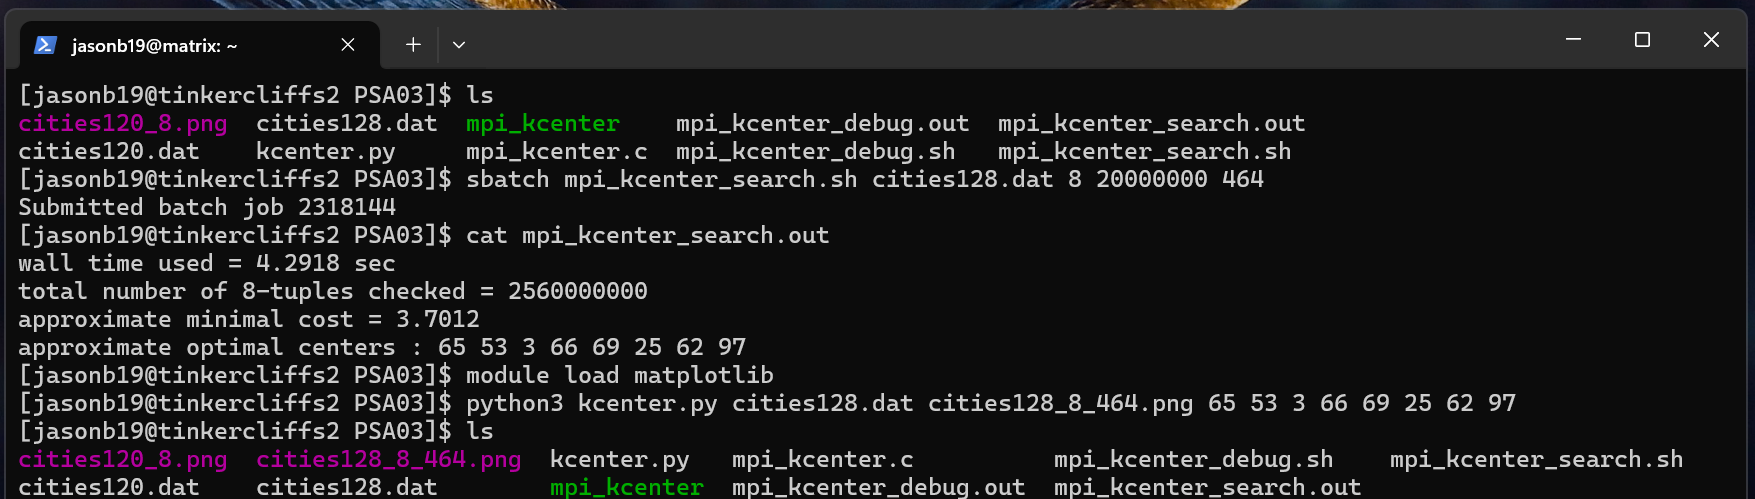
\includegraphics[width=0.95\textwidth]{images/random_num_1.png}
\end{center}
\caption{ARC Command $k$=8, $m$=2M, and $s$=464}
\label{random_num_1.fig}
\end{figure}


Figure \ref{cities128_8_464.fig} is my python image output. This image produces the optimal k-centers for each of the 128 data points given my random seed number as 464.
 
\begin{figure}[H]
\begin{center}
    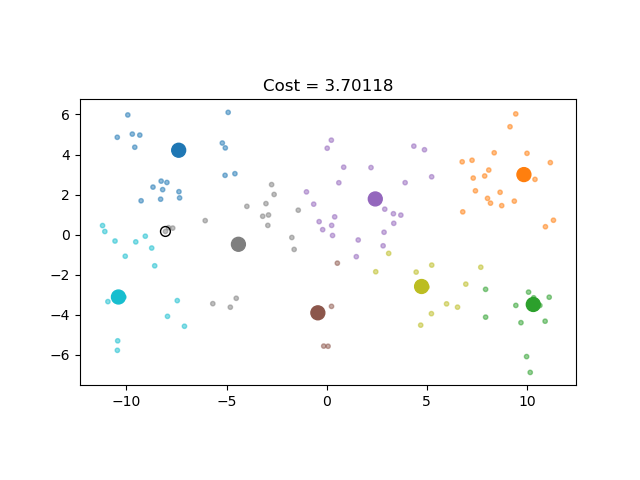
\includegraphics[width=0.95\textwidth]{images/cities128_8_464.png}
\end{center}
\caption{An Optimal Image for $k$=8, $m$=2M, and $s$=464}
\label{cities128_8_464.fig}
\end{figure}

\item Seed Number: 3464

Figure  
\ref{random_num_2.fig} 
shows my command line run to have my output for my second provided random number of seeds. Figure \ref{random_num_2.fig} also show my output values. 
My command prompt outputs are:
\begin{verbatim}
[jasob19@tinkercliffs2 PSA03] 
" "         $ sbatch mpi_kcenter_debug.sh cities128.dat 8 20000000 3464
Submitted batch job 2318144
[jasonb19@tinkercliffs2 PSA03]$ cat mpi_kcenter_debug.out
wall time used = 4.2852 sec
total number of 8-tuples checked = 2560000000
approximate minimal cost = 3.7012
approximate optimal centers : 25 65 97 104 66 53 69 76
\end{verbatim}

\begin{figure}[H]
\begin{center}
    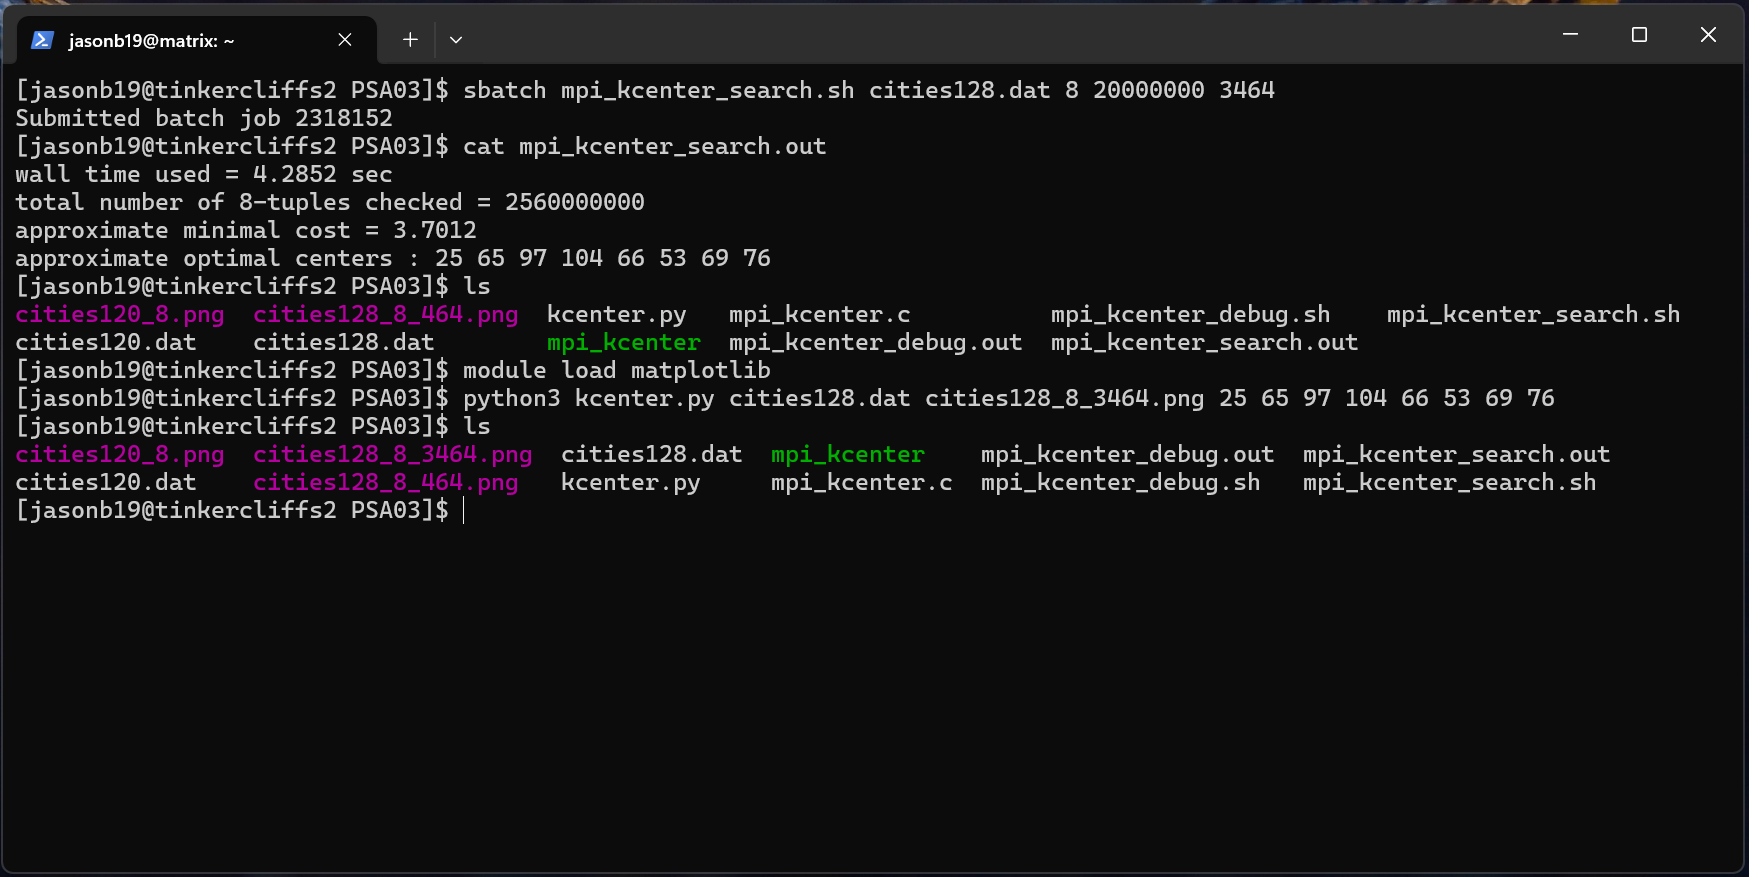
\includegraphics[width=0.95\textwidth]{images/random_num_2.png}
\end{center}
\caption{ARC Command $k$=8, $m$=2M, and $s$=3464}
\label{random_num_2.fig}
\end{figure}


Figure \ref{cities128_8_3464.fig} is my python image output. This image produces the optimal k-centers for each of the 128 data points given my random seed number as 3464.
 
\begin{figure}[H]
\begin{center}
    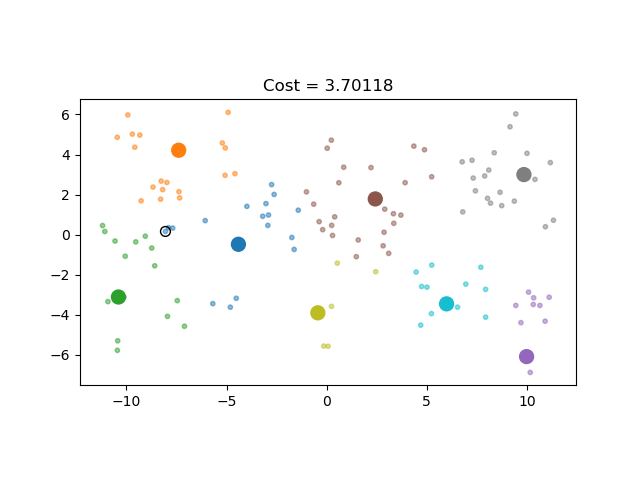
\includegraphics[width=0.95\textwidth]{images/cities128_8_3464.png}
\end{center}
\caption{An Optimal Image for $k$=8, $m$=2M, and $s$=3464}
\label{cities128_8_3464.fig}
\end{figure}

\item Seed Number: 82464

Figure  
\ref{random_num_3_new.fig} 
shows my command line run to have my output for my last provided random number of seeds. Figure \ref{random_num_3_new.fig} also show my output values. 
My command prompt outputs are:
\begin{verbatim}
[jasob19@tinkercliffs2 PSA03] 
" "        $ sbatch mpi_kcenter_debug.sh cities128.dat 8 20000000 82464
Submitted batch job 2318144
[jasonb19@tinkercliffs2 PSA03]$ cat mpi_kcenter_debug.out
wall time used = 4.3042 sec
total number of 8-tuples checked = 2560000000
approximate minimal cost = 3.7012
approximate optimal centers : 46 40 54 97 93 25 53 65
\end{verbatim}

\begin{figure}[H]
\begin{center}
    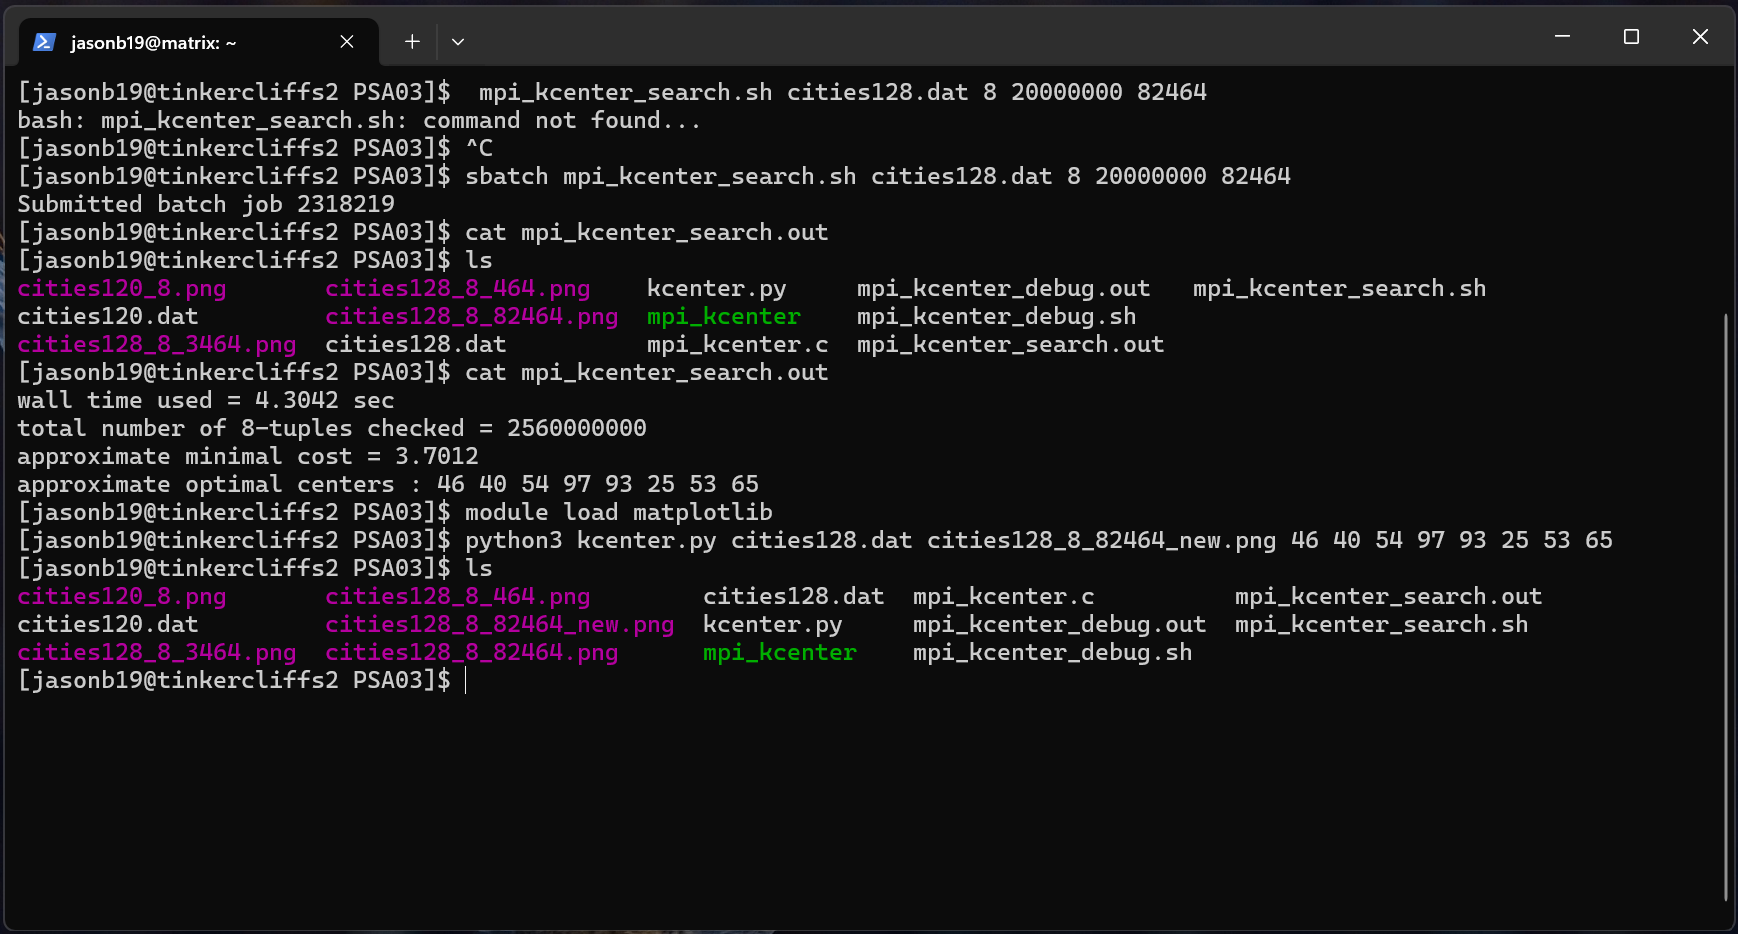
\includegraphics[width=0.95\textwidth]{images/random_num_3_new.png}
\end{center}
\caption{ARC Command $k$=8, $m$=2M, and $s$=82464}
\label{random_num_3_new.fig}
\end{figure}


Figure \ref{cities128_8_82464.fig} is my python image output. This image produces the optimal k-centers for each of the 128 data points given my random seed number as 82464.
 
\begin{figure}[H]
\begin{center}
    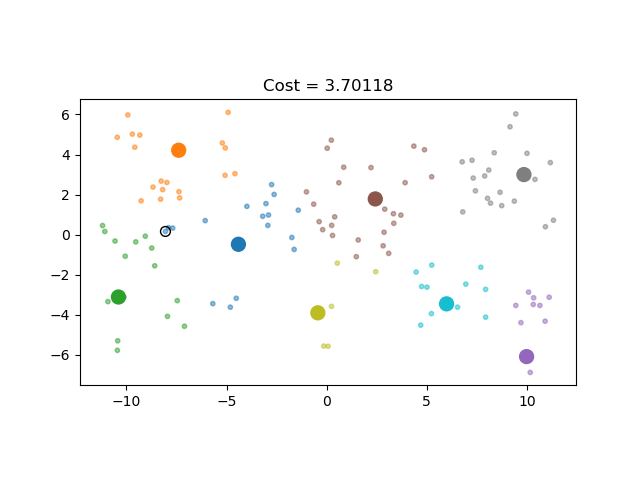
\includegraphics[width=0.95\textwidth]{images/cities128_8_82464.png}
\end{center}
\caption{An Optimal Image for $k$=8, $m$=2M, and $s$=82464}
\label{cities128_8_82464.fig}
\end{figure}

To summarize what I found from my randomly selected seed numbers, I found that they all had the same minimum cost, however, some took a little longer to run. I also found that I had different optimal center outputs. I am not sure if this means anything or there is a similar correlation with many sets of k-centers and our optimal. Hence, there is more than one way to produce the minimal cost but some run quicker by the number of seed input. I would assume that my last random number generated seed would have been the quickest but unfortunately It was slightly slower than my second random number. There for Figure \ref{cities128_8_3464.fig} had the most optimal values for my output, that being, the lowest cost, and the quickest wall time. 

\end{enumerate}


% end of Search Write-Up Tasks 

\end{document}
